\documentclass{article}
\usepackage{amsmath}
\usepackage{mathtext}
\usepackage[T1,T2a]{fontenc}
\usepackage[utf8]{inputenc}
\usepackage[english, bulgarian, russian]{babel}
\usepackage{tikz}
\usepackage{pgfplots}
\usepackage[export]{adjustbox}
\usepackage{siunitx}
\usepackage{booktabs}
\usepackage{pgfplotstable}
\usepackage[left=2cm,right=2cm,
    top=2cm,bottom=2cm,bindingoffset=0cm]{geometry}
    
    
\sisetup{
  round-mode          = places, % Rounds numbers
  round-precision     = 2, % to 2 places
}

\title{Теплоемкость идеального газа и степени свободы его молекул}
\author{Сенчуков Лев}

\begin{document}
  \pagenumbering{gobble}
  \maketitle
  \newpage
  \pagenumbering{arabic}
  
  

\section{Введение}
Из курса молекулярной физики известно, что теплоемкость газа при постоянном объеме
   \begin{equation*}
C_v =\frac {i}{2} R
  \end{equation*} 
зависит от количества степеней свободы молекул, из которых состоит газ, и складывается из тепломкостей соответсвующих различным видам движения молекул:
   \begin{equation*}
C_v = C_{пост} + C_{вращ} + C_{колеб}
  \end{equation*} 
Каждая из степеней свободы молекулы имеет определенную температуру активации, таким образом изохорная теплоемкость газа в общем случае является функцией температуры. При очень низких температурах когда заселены только самые низкие уровни поступательной вращательной и колебательной энергии, можно сказать, что $C_v = 0$. При дальнейшем повышении температуры происходит "размораживание" различных степеней свободы. Сначала происходит активация степени свободы поступательного движения, как правило соответствующая этому температура крайне мала, затем происходит активация степеней свободы поступательного и вращательного движения. Таким образорм, чтобы узнать теплоемкость идеального газа при данной температуре, кам необходимо знать температуры активации его степеней свободы $\Theta_{пост}$, $\Theta_{вращ}$, $\Theta_{колеб}$.
\section{Температура активации степени свободы поступательного движения}
Согласно классической механике энергия частицы может принимать любое значение и меняется непрерывно. Квантовая механика устанавливает дискретный характер изменения энергии частицы, т. е. она может принимать только некоторые фиксированные значения. На практике для выполнения классических представлений достаточно: 
   \begin{equation*}
\frac{\Delta E_i}{k} \ll T
  \end{equation*} 
 Для разных видов движения величина $\Delta E_i$ может быть представлена в виде 
    \begin{equation*}
\Delta E_i = \Delta E \cdot f(i)
  \end{equation*} 
  где $f(i)$ функция, зависящая только от квантовых чисел, а $\Delta E$ - постоянная, характеризующая данный тип движения.
  Величина $\Theta = \frac{\Delta E}{k}$ называется характеристической температурой для данного вида движения. Таким образом, критерий применимости классических представлений:
      \begin{equation*}
T \gg \Theta
  \end{equation*} 
Рассмотрим случай поступательного движения. Чтобы найти разрешенные значения энергии молекулы, поместим ее в сосуд размером $l_x \cdot l_y \cdot l_z$.
Её движение будет описываться уравнением Шредингера:
      \begin{equation*}
-\frac{h^2}{8 \pi^2m}\big(\frac{\partial^2 \Psi}{\partial x^2}+\frac{\partial^2 \Psi}{\partial y^2}+\frac{\partial^2 \Psi}{\partial z^2}\big) = (E - П)\Psi
  \end{equation*} 
  Где квадрат модуля $\Psi$ - плотность вероятности нахождения частицы в заданном объеме, i - целое положительное число. Так как газ идеальный, П = 0, а решение уравнения Шредингера даст нам допустимые значения энергии:
        \begin{equation*}
E_i = E_{xi} + E_{yi} + E_{zi}=\frac{h^2}{8m}\big(\frac{i_x^2}{l_x^2}+\frac{i_y^2}{l_y^2}+\frac{i_z^2}{l_z^2}\big)
  \end{equation*} 
  В случае, если мы рассматриваем движение вдоль одной из координат:
\begin{equation*}
(\Delta E_x)_i = \frac{h^2}{8l_x^2m}(2i_x+1) = \frac{h^2N_A}{8l_x^2M}(2i_x+1)
\end{equation*} 
Тогда характеристическая температура поступательного движения равна:
\begin{equation*}
\Theta_{пост} = \frac{h^2N_A}{8l_x^2M} = \frac{\Delta E}{k}
\end{equation*} 
Что бы определить порядок ее величины, вычислим ее для молекулы азота при размерах системы порядка 1 см. 
\begin{equation*}
\Theta_{пост} = \frac{(6,63\cdot 10^{-34})^2 \cdot 6,02 \cdot 10^{23}}{8\cdot 10^{-4}\cdot 28 \cdot 10^{-3}\cdot 1,38 \cdot 10^{-23}} \approx 10^{-18} К
\end{equation*} 
Это значит, что практически для всех температур $T \gg \Theta_{пост}$, и вклад поступательного движения в теплоемкость всегда классический, 1,5R.
\section{Температура активации степени свободы вращательного движения}
Согласно классической механике:
\begin{equation*}
E{вращ} = \frac{M^2}{2J}
\end{equation*}
Формула сохраняется в квантовой механике, с той лишь разницей, что M может принимать только определенные значения $M = \frac{h}{2\pi}\sqrt{j(j+1)}$. Тогда:
\begin{equation*}
E{j} = \frac{h^2}{8\pi^2J}\cdot j(j+1)
\end{equation*}
Тогда характерная величина вращательной температуры:
\begin{equation*}
\Theta{вр} = \frac{h^2}{8\pi^2Jk} =  \frac{h^2N_A}{8\pi^2Mr^2k}
\end{equation*}
Вычислив значение данной величины для молекулы водорода, получим:
\begin{equation*}
\Theta{вр} \approx 87 К
\end{equation*}
Для более крупных молекул данная величина можеть быть ниже более, чем на порядок. Поэтому даже при не очень высоких температурах можно пользоваться классическим приближением при рассчете энергии вращения.
Именно данная формула объясняет тот факт, что степень свободы вращения молекулы вокруг собственной оси практически никогда не может быть активирована, ведь 
\begin{equation*}
\Theta{вр}  \sim  \frac{1}{r^2}
\end{equation*}
Таким образом для водорода данная степень свободы акивируется при температуре порядка $10^{11} К$ , что в $10^{7}$ раз больше температуры поверхности Солнца.
\section{Температура активации степени свободы вращательного движения}
Нелинейная молекула представляет собой (3n-6), линейная (3n-5) гармонических осциллятора, частоты колебания которых лежат в пределе $10^{12}-10^{14} c^{-1}$. Тогда соответствующая величина $\Delta E$:
\begin{equation*}
\Delta E = h \nu
\end{equation*}
Тогда характеристическая колебательная температура равна:
\begin{equation*}
\Theta_{кол} = \frac{h \nu}{k} \approx 50-5000 К
\end{equation*}
Для большинства молекул $\Theta_{кол}$ лежит в интервале 1500-4000 К, то есть почти все молекулы находятся в невозбужденном состоянии, и только при очень высоких температурах вклад колебаний в теплоемкость составляет $\sim$ R.
\section{Изменение теплоемкости с ростом температуры}
Таким образом, мы можем сказать, как теплоемкость идеального газа зависит от температуры:\\
Начиная уже с $10^{-18}$ К происходит активация поступательных степеней свободы и теплоемкость тела становится равной $\frac{3}{2}$R. Затем при температуре порядка 10 К происходит возбуждение вращательных степеней свободы: 2 у линейных молекул (возбуждение 3 не происходит ввиду малости момента инерции соответствующего третьей оси вращения) и 3 у нелинейных, каждая из которых увеличивает теплоемкость на $\frac{1}{2}R$, при температурах от 1500-4000 К происходит возбуждение колебательных степеней свободы, каждая из которых вносит вклад от 0 до R.
\section{Представление зависимости теплоемкости от температуры}
Обычно результаты теоретического рассчета или экспериментальных данных представляют в виде
\begin{equation*}
C_v = a+bT+cT^2
\end{equation*}
или
\begin{equation*}
C_v = a+bT+\frac{c}{T^2}
\end{equation*}
Коэффициенты определяются эмпирически и могут быть найдены в термодинамических справочниках.
Практическая важность определения температур активации различных степеней свободы молекулы проявляется при работе с системами, температура которых во время работы может значительно меняться. Представленные выше формулы могут с определенной точностью предсказать те температуры, при которых изохорная теплоемкость системы изменится.Также мною были построены графики (1 - теоретический, 2 - экспериментальный):
         \begin{center}
  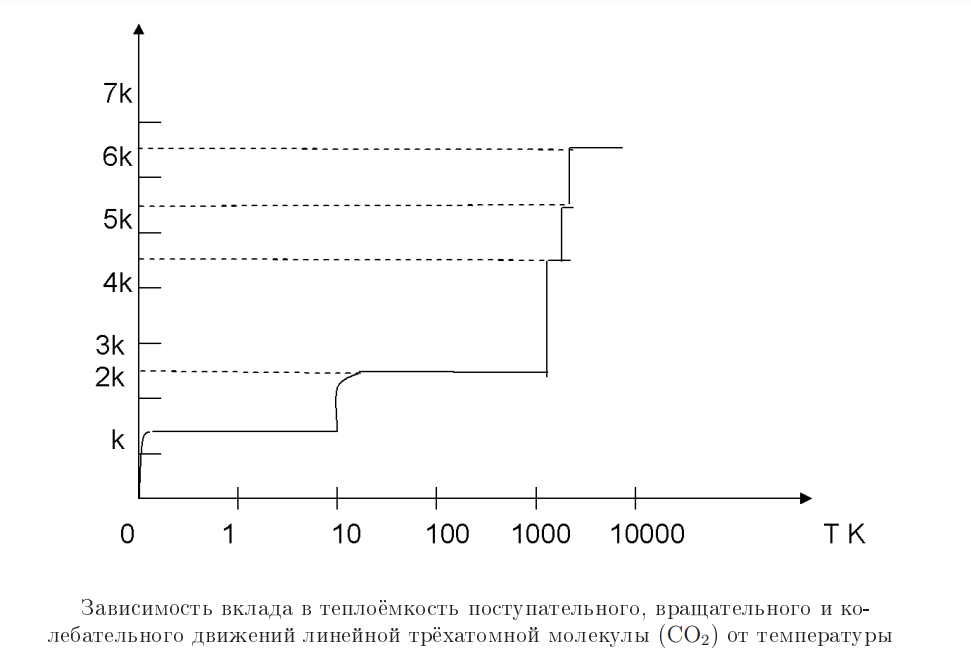
\includegraphics[width=0.8\linewidth]{ooh.png}\\
 \end{center}
          \begin{center}
  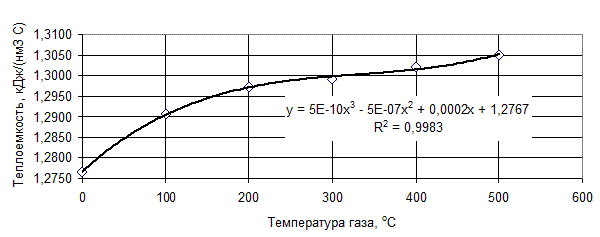
\includegraphics[width=0.8\linewidth]{hoo.png}\\
 \end{center}
 На экспермиентальном явно видны изгибы графика, соответствующие возрастанию теплоемкости, также график начинается не из 0, что показывает, что теплоемкость начинает возрастать при очень низких температурах. Практическое значение исследований теплоемкости важно для расчетов энергетических балансов процессов в химических реакторах и других аппаратах химического производства, а также для выбора оптимальных теплоносителей. 
\end{document}
